\documentclass[12pt]{article}

% This is the preamble, load any packages you're going to use here
% \usepackage{physics} % provides lots of nice features and commands often used in physics, it also loads some other packages (like AMSmath)
\usepackage{siunitx} % typesets numbers with units very nicely
\usepackage{enumerate} % allows us to customize our lists
\usepackage{hyperref}
\usepackage{xcolor}
\usepackage{graphicx}
\usepackage[version=4]{mhchem}
\usepackage{siunitx}
\usepackage{enumitem}
\usepackage[most]{tcolorbox}
\tcbuselibrary{skins}
\newtcolorbox{explorationbox}[1][]{%
  enhanced,
  colback=blue!10,
  colframe=blue!50!black,
  fonttitle=\bfseries,
  left=20pt,
  title=Questions for further exploration:,
  #1
}
\newtcolorbox{warningbox}[1][]{%
  enhanced,
  colback=red!10,          % Light reddish background
  colframe=red!50!black,   % Darker red frame
  fonttitle=\bfseries,
  title=Warning:,          % Title of the box
  #1
}


\begin{document}

\title{Exploring the Algorithmic Instructions Sufficient for Thermalization in Gas Phase}
\author{Anton Morgunov}
\date{\today}

\maketitle

% \begin{abstract}

% \end{abstract}

\section{Motivation}
In statistical mechanics, we try to derive macroscopic variables through properties of individual components such as atoms or molecules. Those macroscopic variables, however, are end results (after all, there is no concept of time in thermodynamics). I was interested in the mechanism by which that \textit{end result} is achieved. Particularly, I was interested to see what kind of instructions should I encode for two kinds of particles (potentially with different masses and temperatures), initially placed in different compartments of a box to a) diffuse b) thermalize. 

\begin{warningbox}
    Both the simulation code and this report are work in progress
\end{warningbox}

Also, note that because this is a description (or reflection on) of an educational experience, I will include chronological description of my thought process and the steps I took to get to the final result.

\section{Methods}
\subsection{Initialization Parameters}
The \texttt{constants.py} file contains all the parameters that are used in the simulation: box dimensions, initial temperature, number of particles, etc.

\subsection{Data Structures}
I define a class \texttt{Particle} which stores particle position $(x,y)$ and velocities $v_x,v_y$. Coordinates $(x,y)$ are drawn independently from a uniform distribution defined by the compartments of the box. Initially, I modeled random walk in which velocities $v_x$ and $v_y$ are independently drawn from a uniform distribution $[-1,1]$. Then, I decided to model the behavior of particles in a gas phase. In the gas mode, velocities are initialized as $v_x=v_0 \cos \phi$ and $v_y=v_0 \sin \phi$ where $v_0$ is the initial velocity (defined in \texttt{constants.py}, constant for all particles) and $\phi=2\pi n$ where $n$ is drawn from a uniform distribution $[0,1]$. An important method of the Particle class is \texttt{move} which updates the position of the particle according to its velocity:
\begin{align}
    x_t &= x_{t-1} + v_x & y_t &= y_{t-1} + v_y
\end{align}
Right now, \texttt{move} method also reflects the velocity components if the particle hits the wall. Another important method is \texttt{check\_collisions}. This method checks if the particle collides with another particle, and if it does, computes new velocities for both particles by treating the collision as perfectly elastic.

I also define a class \texttt{Game} which stores a list of \texttt{Particle} objects. Game class has a \texttt{timestep} method, which calls the \texttt{move} method for each particle, then tries to resolve collisions if there are any by calling the \texttt{check\_collisions}. There is a trivial $O(n^2)$ algorithm (which results in the simulation being practical only for up to 200 particles) and a smarter check which distributes particles on the \texttt{Grid} (defined as separate class) and only checks for collisions between particles that are in the same cell or neighboring cells.

\texttt{Game} method has an \texttt{export} method which exports the current state of the game into a python dictionary. In addition, there are methods:
\begin{enumerate}
    \item \texttt{update\_compartment\_fractions}. Computes fraction of particles of second kind in left and right compartments.
    \item \texttt{compute\_velocity\_distribution}. Computes the distribution (as a histogram) of $v_x^2$, $v_y^2$, and $v_x^2+v_y^2$.
    \item \texttt{find\_equipartition\_temperature}. Computes the temperature according to:
    \begin{align}
        \langle KE \rangle = \frac{3}{2} k_B T = \frac{1}{2} m \sum_i v_i^2 \implies T = \frac{m}{3k_B N} \sum_i v_i^2
    \end{align}
\end{enumerate}

\subsection{Simulation Visualization}

I use a \texttt{Flask} library to create a server, which provides several endpoints:
\begin{enumerate}
    \item \texttt{/game\_state} which calls the \texttt{timestep} method of \texttt{Game} class
    \item \texttt{/game\_reset} which reinitializes the game.
    \item \texttt{/game\_analyze} which exports the evolution of temperature and compartment fractions as a function of timestep as Plotly figures.
\end{enumerate}

These endpoints are called by the \texttt{index.html} file, which uses \\\texttt{JavaScript} to~populate the \texttt{HTML} canvas with the current state of the game. In addition, the velocity distributions, compartment fractions, and current temperatures are plotted using \texttt{Chart.js}.
    
% Being Cautious \href{https://en.wikipedia.org/wiki/Anscombe%27s_quartet}{\textcolor{blue}{Anscombe's Quartet}}

\section{Results}
\subsection{Preliminary Exploration with Random Walk}
At first, I created $n=200$ particles with identical mass $m=\qty{1}{amu}$ and launched the random walk. The box was large enough for practically all particles move in a small area around their initial position, never meeting other particles.

\begin{explorationbox}
    From what distribution should I draw the initial velocities to properly model Brownian Motion? That is, what is the interval and how is the probability distributed within that interval? 
\end{explorationbox}

At some point, I started wondering: why are we even considering random walk? How can a particle move with one velocity and then at the next step abruptly change it? If the particle changes not just the direction but also the magnitude of velocity, that clearly violates the conservation of momentum. The abrupt change in direction is unrealistic because it implies infinite acceleration. I started reading more about the Brownian motion and, to my embarassment, realized that I confused the appearance of a mechanism for the mechanism itself. In other words, it only seems that particles are moving in a random walk, but there's nothing random about the walk of each particle. The \textit{abrupt} changes in direction are actually the result of collisions with other particles.

That's how I ended up implementing the $v_x=v_0 \cos\phi$ and $v_y=v_0 \sin \phi$ velocity initialization scheme. I also created the collision resolution method, which treats all collisions as perfectly elastic. To my surprise, I started seeing that some particles started to move slower, and some particles started to move faster. After sufficient timesteps, the distribution of speeds started to resemble the Maxwell-Boltzmann distribution. This seems to imply that the mechanism for thermalization is the collisions between particles.

\begin{warningbox}
    As we will see shortly, there are reasons to believe that I have bugs/mistakes in the current implementation of the collision algorithm. If that's the case, it may turn out that the correct implementation of the collision algorithm will not result in the Maxwell-Boltzmann distribution.
\end{warningbox}
\begin{figure}[ht]
    \centering
    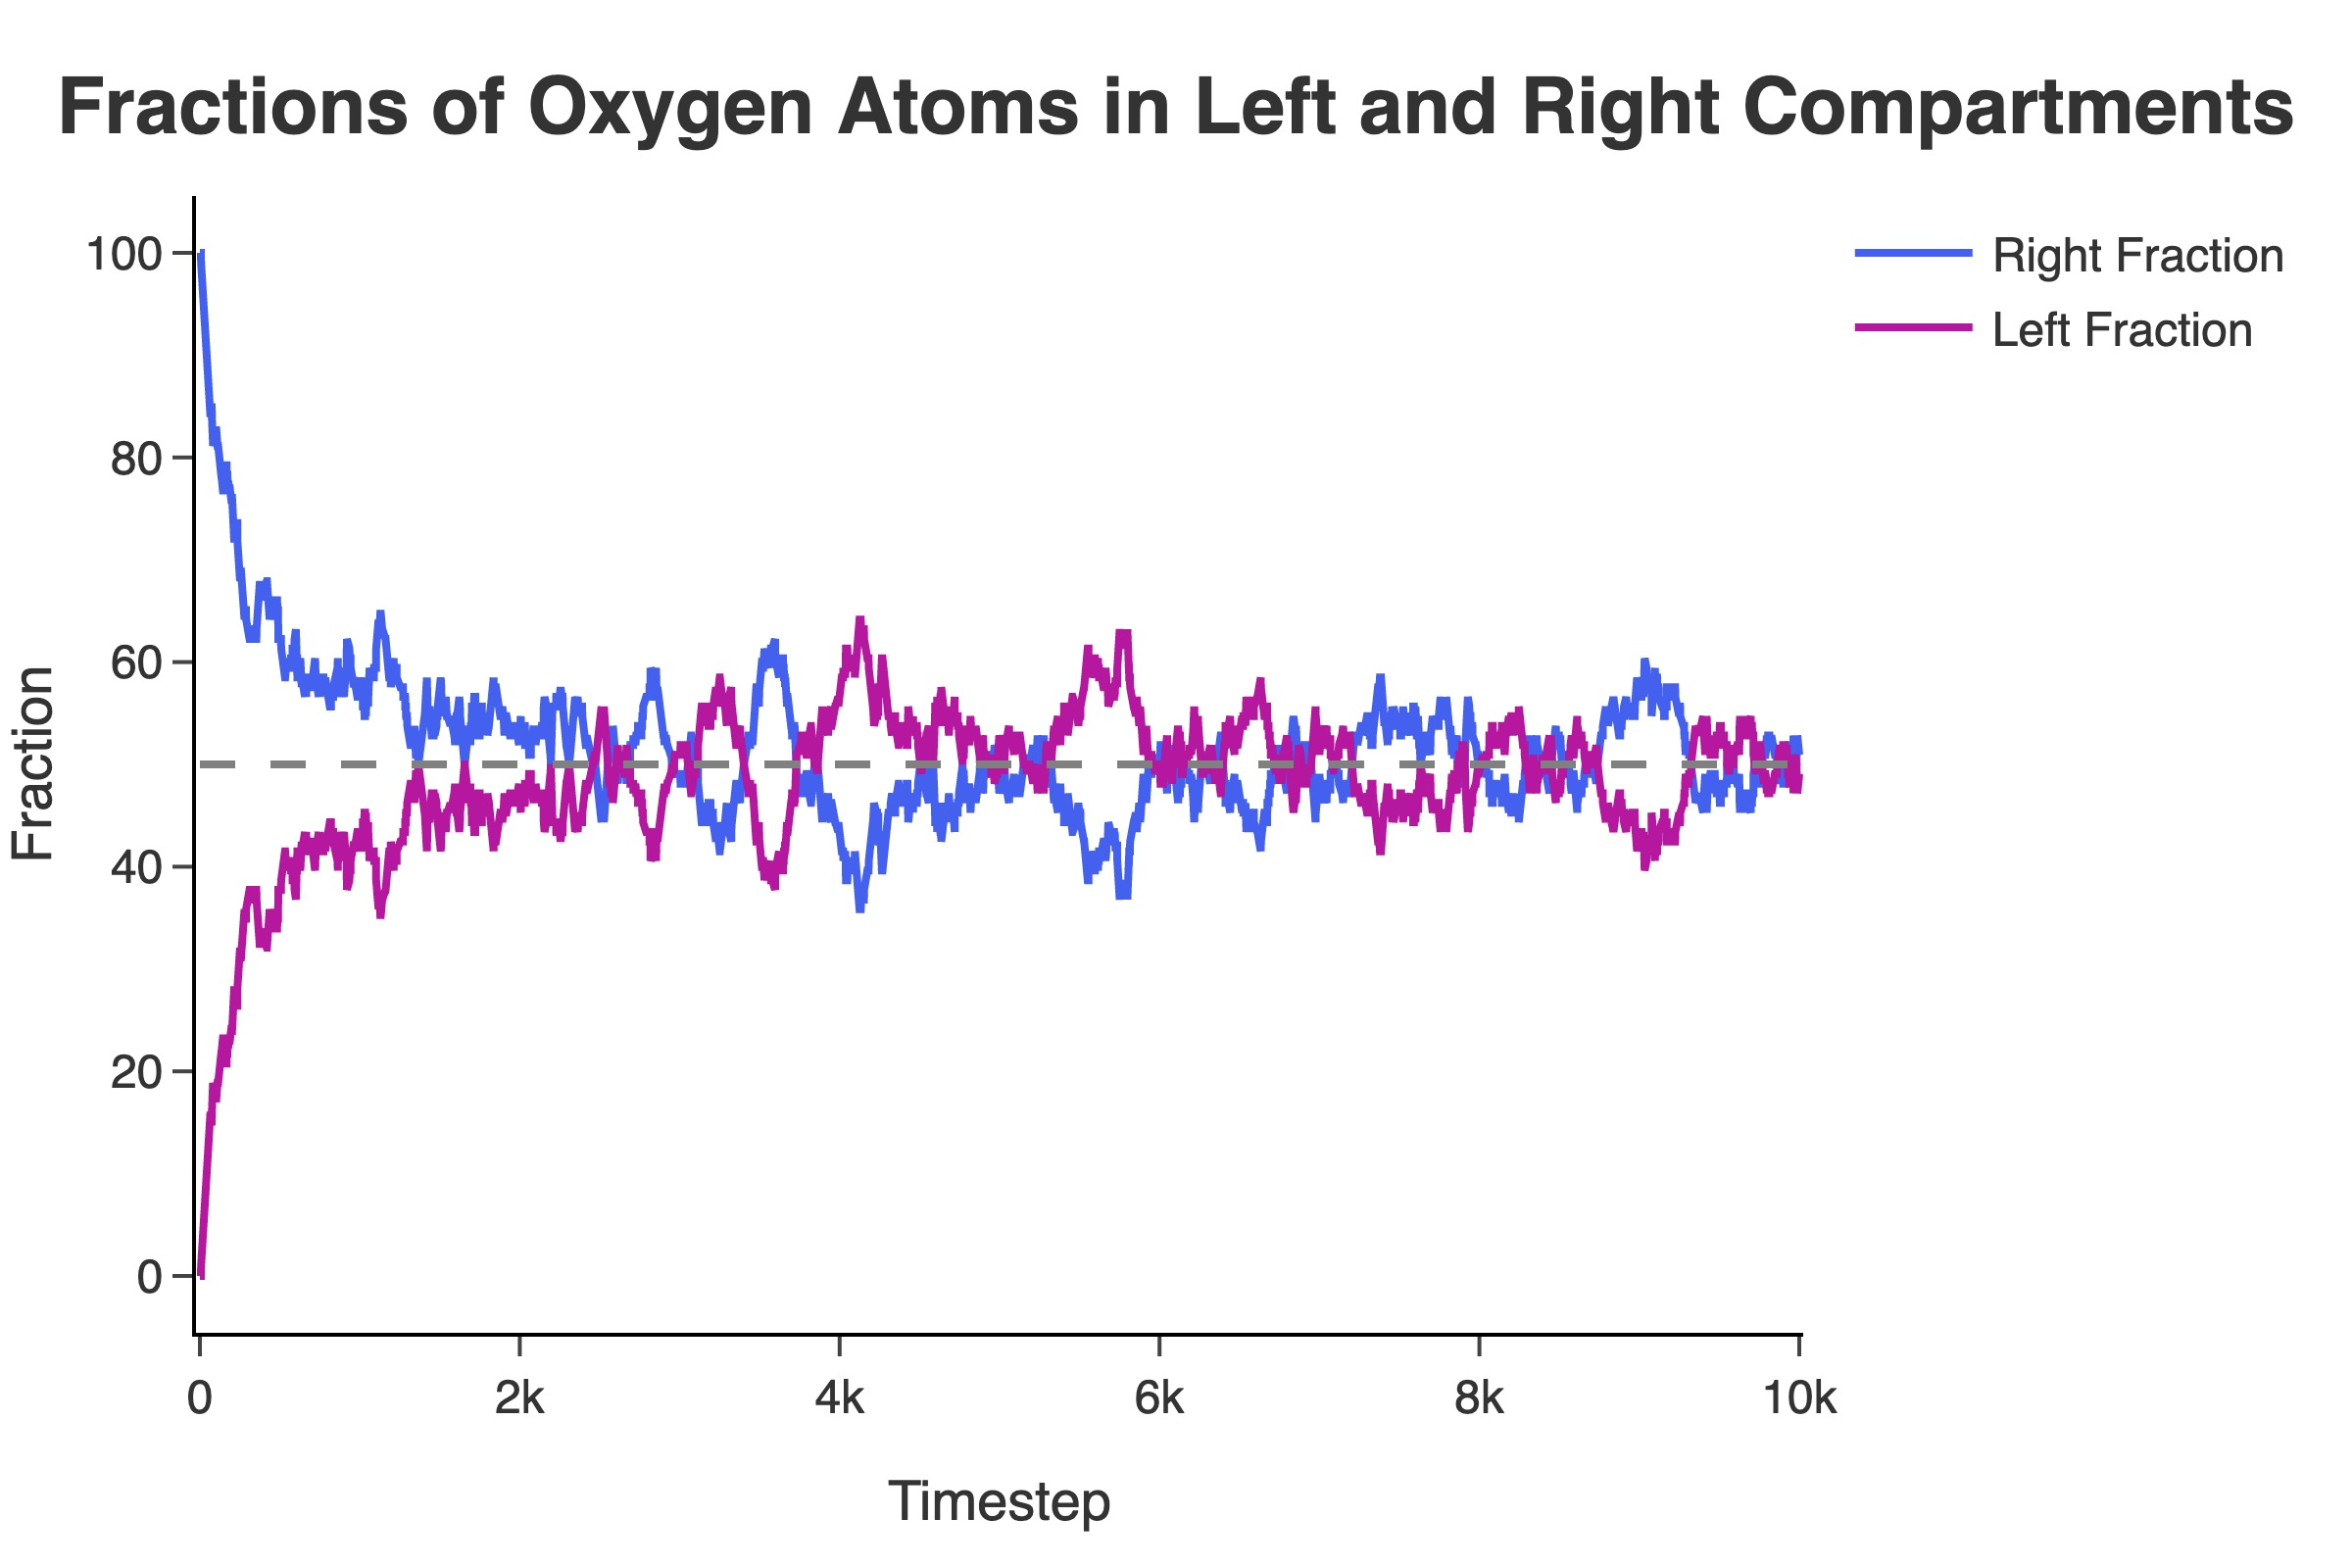
\includegraphics[width=0.8\linewidth]{../figures/jpg/n200_m1_10k/compartment_fractions.jpg}
    \caption{Evolution of compartment fractions}
    \label{fig:compartment_fractions}
\end{figure}

\begin{figure}[h]
    \centering
    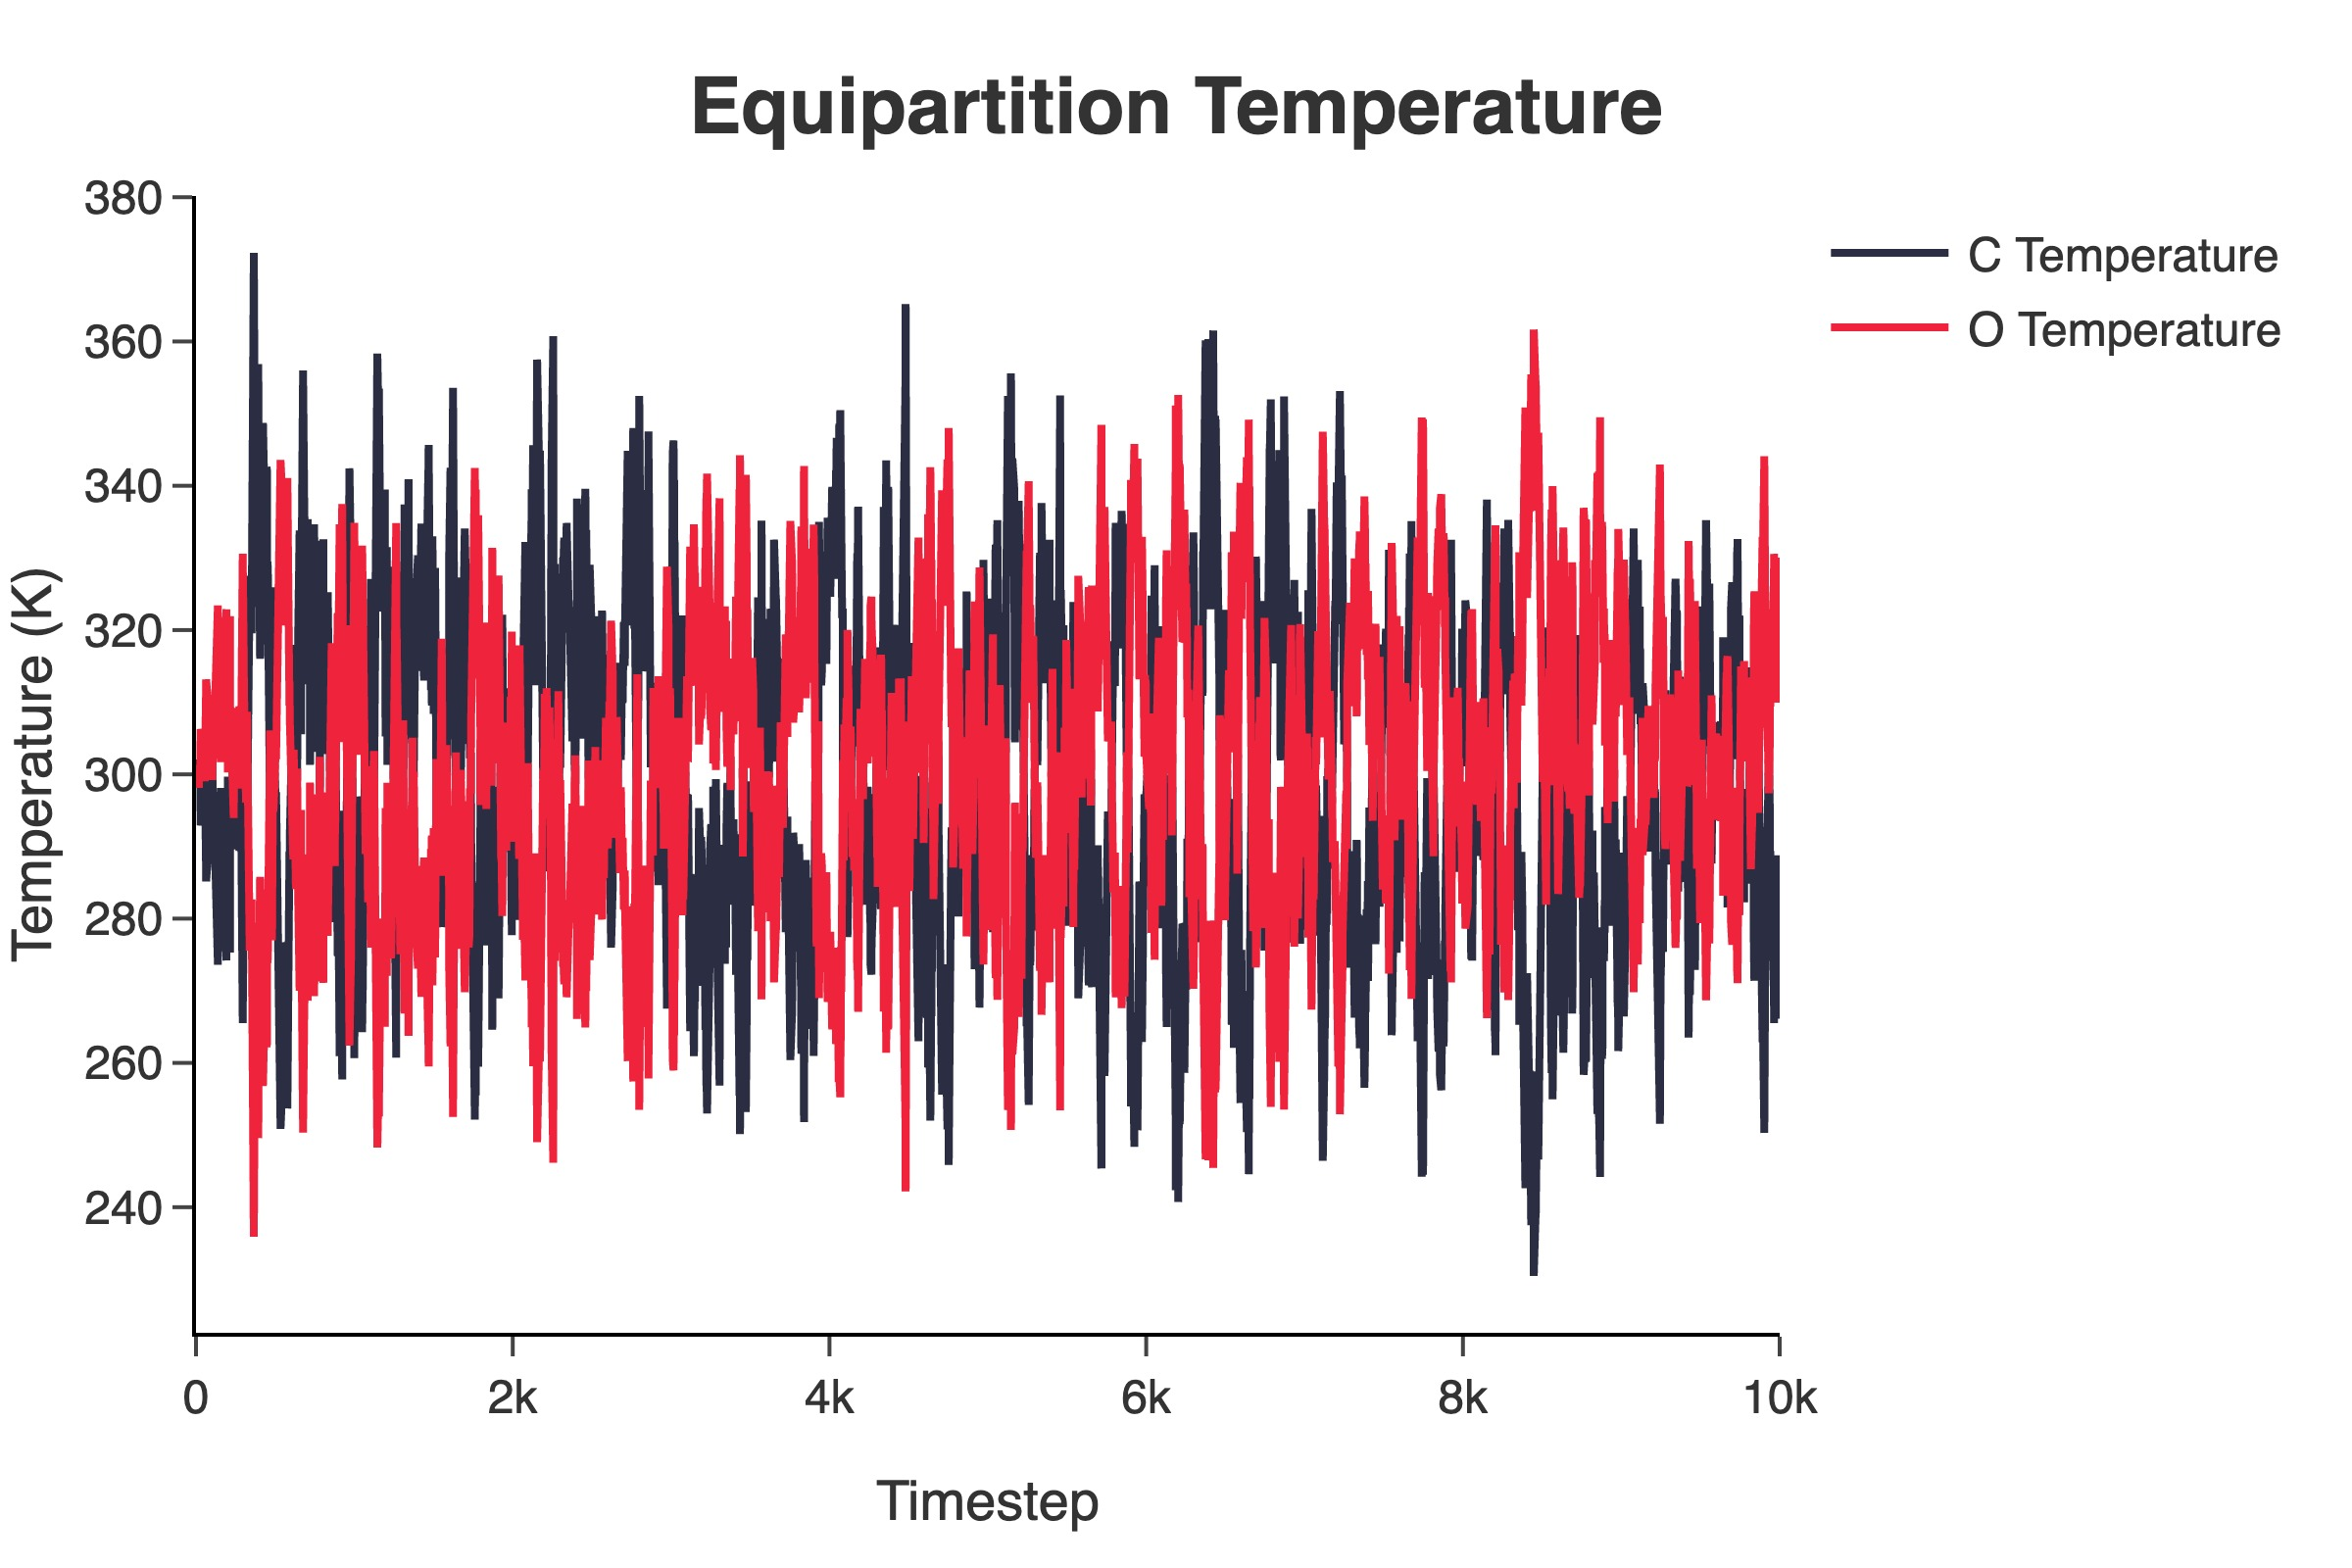
\includegraphics[width=0.8\linewidth]{../figures/jpg/n200_m1_10k/equipartition_temperature.jpg}
    \caption{Evolution of temperature}
    \label{fig:temperature}
\end{figure}

\subsection{Identical particles}
If we set both kinds of particles to have $m=1$ and initial temperature
$T=\qty{300}{K}$, and create $n=200$ of those, we can see that particles diffuse and thermalize (Figures \ref{fig:compartment_fractions} and \ref{fig:temperature}). Somewhat not surprisingly, the average temperature of the system is near $T=\qty{300}{K}$, but fluctuates quite significantly.


\subsection{Different masses}
One of my primary objectives was to fill the left compartment of the box with, say, carbon atoms at $T_1$ and the right compartment with, say, oxygen atoms at $T_2$, and see whether/how the two sets of particles thermalize. The choice of elements is superficial, it's suffice to choose two elements with different masses (perhaps H and He would be a better choice). Importantly, $T_1\neq T_2$. If the final temperature matches the one predicted by the heat transfer equation, that would further solidify the idea that the mechanism for thermalization is the collisions between particles.

Unfortunately, when I fill the compartments even with $T_1=T_2=\qty{3000}{K}$ (such high temperature is chosen for particles to move fast enough), after some timesteps the temperature starts to blow up (Figure \ref{fig:temperature-explosion}). Obviously, this indicates that there has to be a bug in my code, and I suspect it has to do with the collision resolution algorithm. As much as I'm tempted to keep digging until I resolve this, I have to postpone it.

\begin{figure}[h]
    \centering
    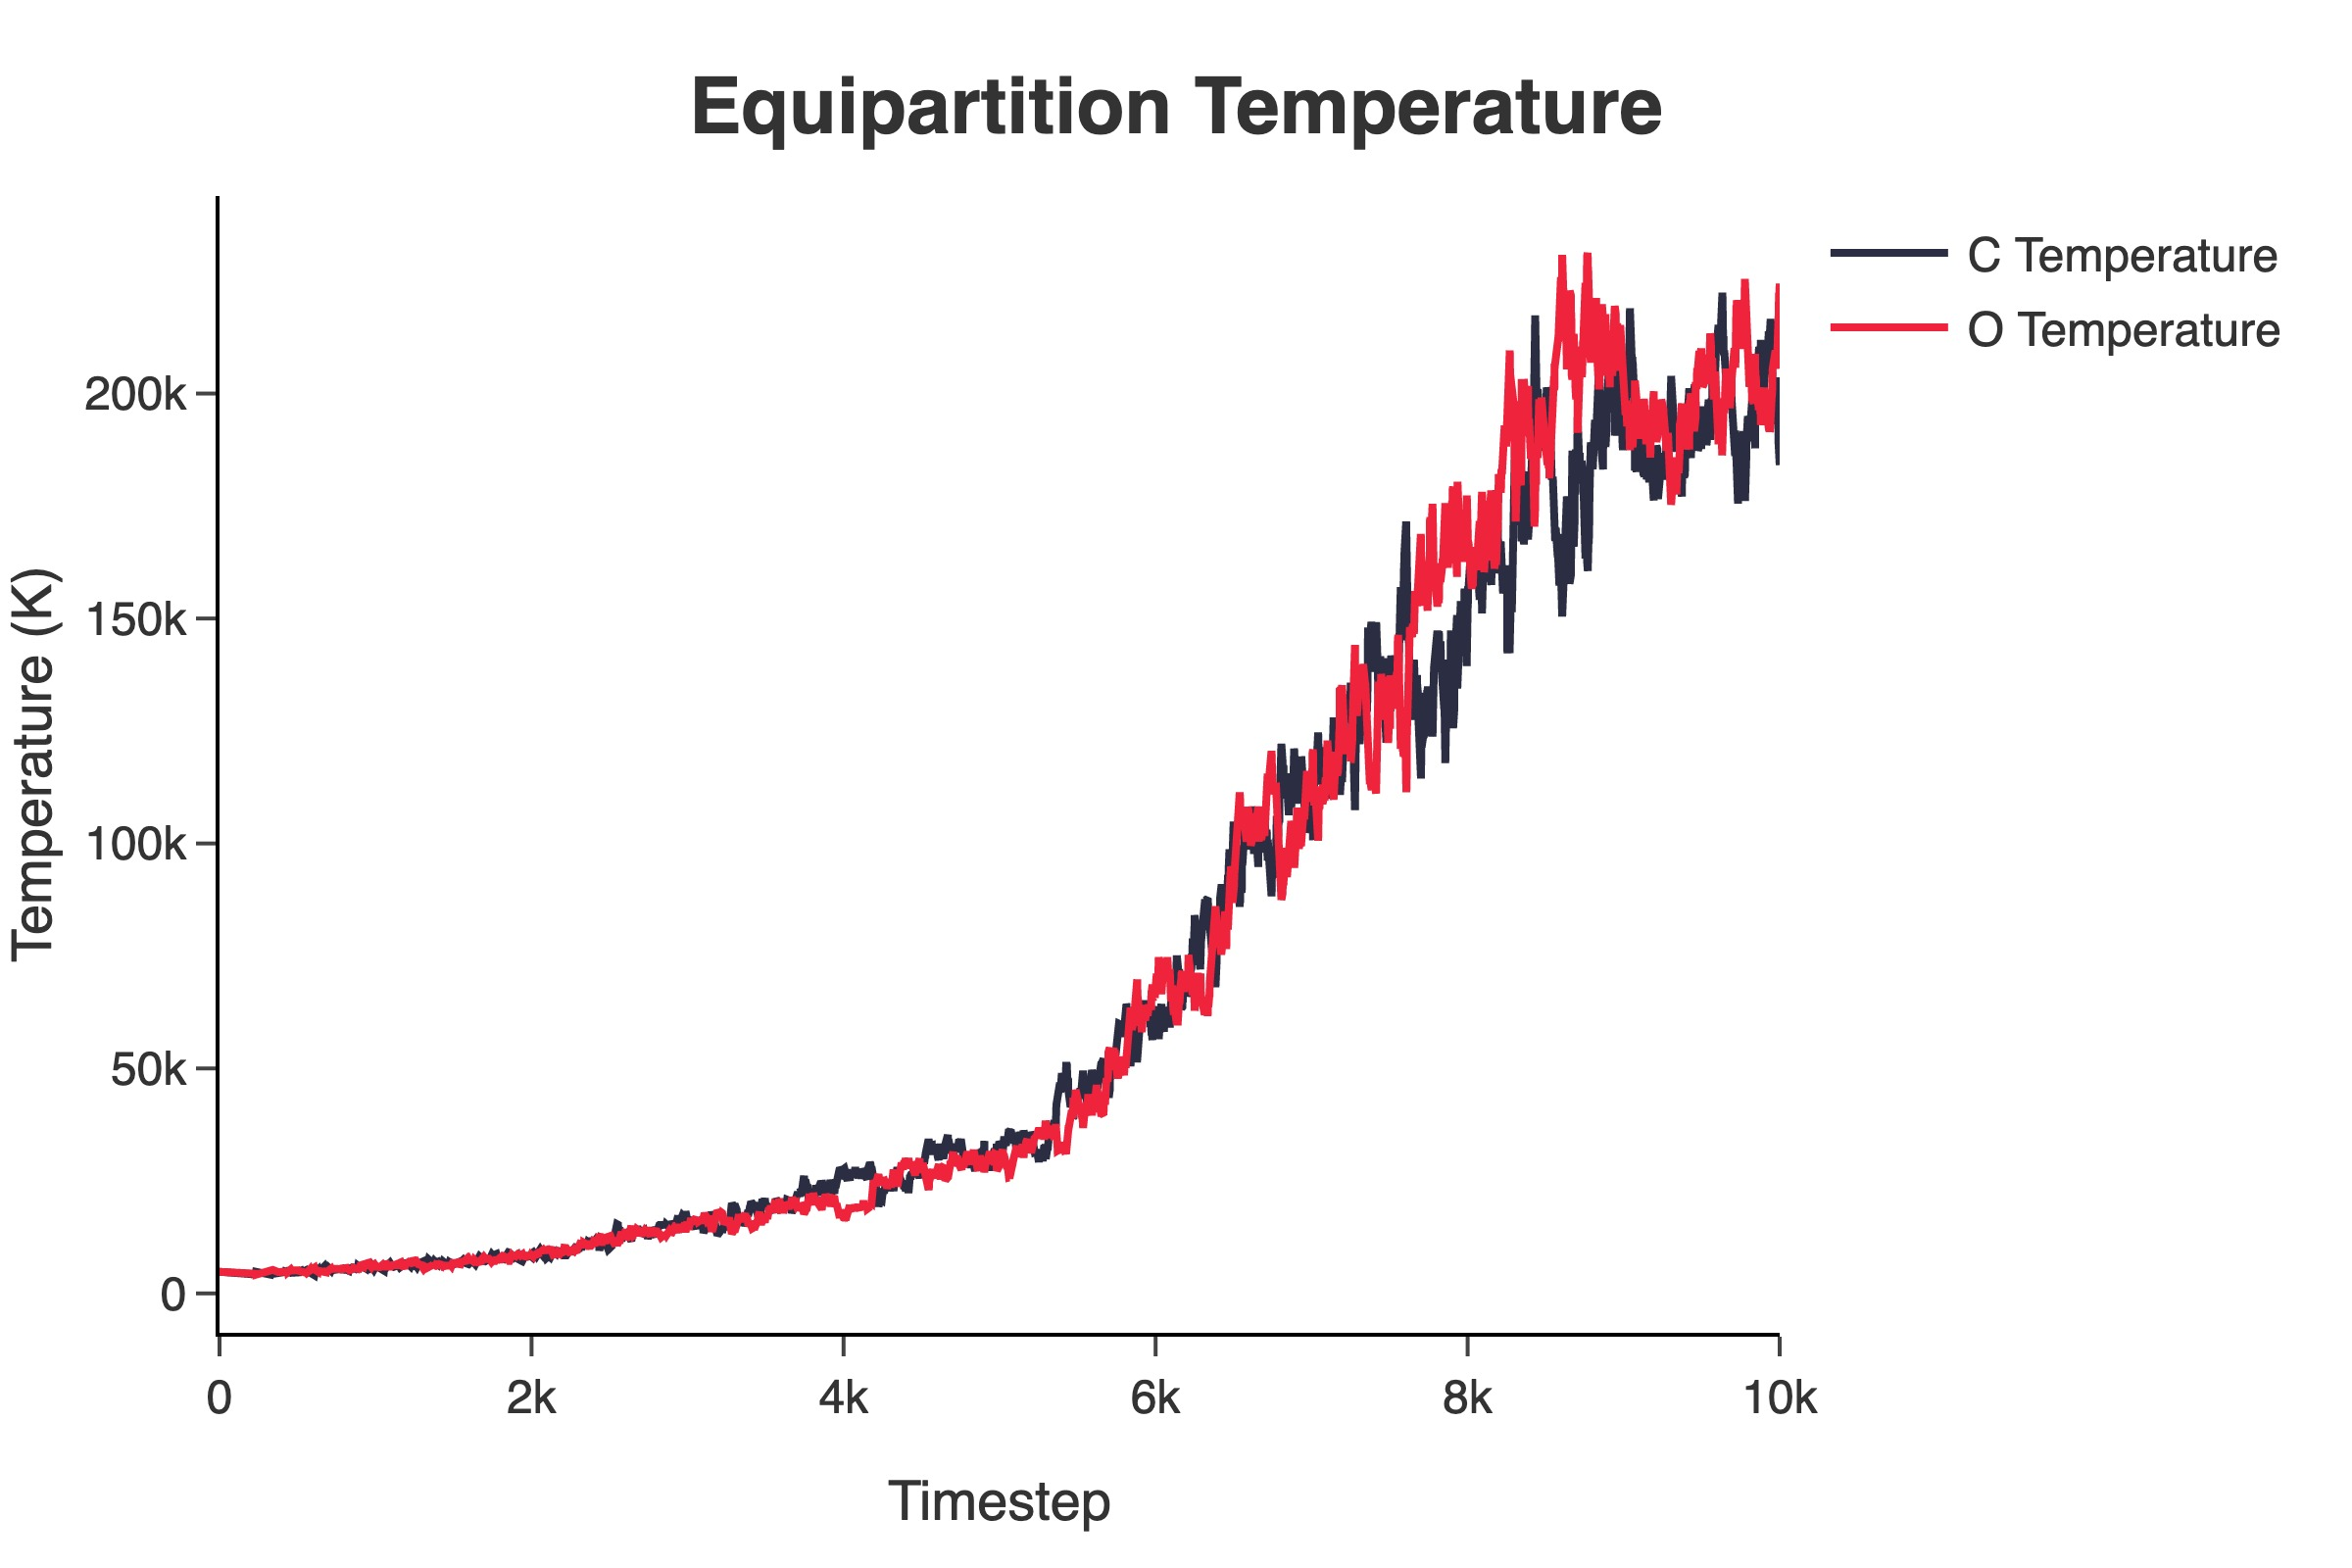
\includegraphics[width=0.8\linewidth]{../figures/jpg/equipartition_temperature_explosion.jpg}
    \caption{Explosion of Temperature when particles of different masses are introduced}
    \label{fig:temperature-explosion}
\end{figure}

\section{Future Work}
Here's a list of tasks I could potentially do:

\begin{enumerate}
    \item Find the mistake in the simulation algorithm
    \item Expand the UI of the simulation to allow for more customization: choosing elements, initial temperatures, numbers of atoms. 
    \item Perform the simulation (once implemented correctly) with different number of particles and see whether the magnitude of fluctuations in temperature scales as $1/\sqrt{N}$.
    \item Perform the simulation with different initial temperatures and see whether the final temperature matches the one predicted by the heat transfer equation.
    \item Investigate inelastic collisions.
    \item Introduce the potential energy term into the simulation. That is, add interatomic interactions.
    \item Trace a trajectory of movement of a single particle in the box.
    \item Make particles to have non-zero volume. I.e. have particles with different sizes.
    \item Explore whether we can model chemical reactions.
    \item Introduce unit tests for significant parts of the code.
    \item Improve documentation.
\end{enumerate}



\end{document}